\documentclass[10pt]{article}
\usepackage{a4}
\usepackage{epsfig}
\usepackage{listings}
\usepackage{tabularx}
\lstset{language=Delphi}%
\lstset{basicstyle=\sffamily\small}%
\lstset{commentstyle=\itshape}%
\lstset{keywordstyle=\bfseries}%
%\lstset{blankstring=true}%
\newcommand{\file}[1]{\textsf{#1}}
\newcommand{\var}[1]{\texttt{#1}}
\usepackage[pdftex]{hyperref}
\newif\ifpdf
\ifx\pdfoutput\undefined
  \pdffalse
\else
  \pdfoutput=1
  \pdftrue
\fi
\begin{document}
\title{Programming GTK in Free Pascal: Using GDK}
\author{Florian Kl\"ampfl\\and\\Micha\"el Van Canneyt}
\date{July 2001}
\maketitle
\section{Introduction}
In this article, some of the graphics primitives from the gdk toolkit will
be demonstrated in a small game - breakout.

The GTK toolkit widgets are built upon the GDK: Graphics Drawing Kit. 
The GDK does not know anything about buttons, menus checkboxes and so on.
Instead, it knows how to create windows, draw on them, handle mouse clicks
and keypresses. This functionality is used by the GTK widget set to create
usable widgets.

Sometimes, the widgets offered by GTK are not enough, and one has to fall
back on the graphics functionality of the GDK to be able to do what is 
needed for a program.

Fortunately, it is not necessary to create a GTK window and handle all
GDK events to be able to use the GDK functions. The GTK widget set has a
special widget, which can be used to draw upon. This widget is the 
\var{TGtkDrawingArea} widget. The use of the \var{TGtkDrawingArea} is what
will be explained below.

The GDK graphics functions will be explained using a simple arcade game,
to demonstrate that the speed of the GDK is sufficient for the creation of
simple games. The breakout game is chosen because it is conceptually simple, 
requires moving graphics and can be extended in many ways.

\section{The drawing area widget}
The drawing area widget (\var{TGTKDrawingArea}) is a simple widget which
just provides a drawing window. It responds to all widget events, and adds
additionally the 'configure\_event', which is called when the widget is
realized (i.e. when the window handle is created.)

The widget has only 1 method: \var{gtk\_drawing\_area\_size}, which sets
the size of the drawing area. It is defined as follows:
\begin{lstlisting}{}
procedure gtk_drawing_area_size(Area:PGtkDrawingArea;
                                width,height:gint)
\end{lstlisting}{}
The arguments to this function are self-explaining.

To use the drawing area widget, one should respond to the 'expose\_event'.
This event is triggered whenever a part of the window that was invisible,
becomes visible. The event handler gets an \var{PGDKEventExpose} parameter,
which describes which area was exposed. This can be used for optimization
purposes.

To draw in the drawing area widget, the \var{Window} field of the
\var{TGTKWidget} parent can be used. This is of type \var{TGDKWindow}.
All drawing functions require a parameter of type \var{TGdkDrawable}
which can be one of the \var{TGdkWindow} or \var{TGdkPixMap} types.

\section{Graphics contexts}
Most drawing functions do not only require a drawable to draw on, they also
require a {\em Graphics Context}. A graphics context is a series of
parameters that determine how lines are drawn, what colors and font are
used etc.

The Graphics Context is an opaque record, and its members cannot be
accessed. The relevant parameters are set in a \var{TGdkGCValues} record,
which is defined as follows:
\begin{lstlisting}{}
foreground : TGdkColor;
background : TGdkColor;
font : PGdkFont;
thefunction : TGdkfunction;
fill : TGdkFill;
tile : PGdkPixmap;
stipple : PGdkPixmap;
clip_mask : PGdkPixmap;
subwindow_mode : TGdkSubwindowMode;
ts_x_origin : gint;
ts_y_origin : gint;
clip_x_origin : gint;
clip_y_origin : gint;
graphics_exposures : gint;
line_width : gint;
line_style : TGdkLineStyle;
cap_style : TGdkCapStyle;
join_style : TGdkJoinStyle;
\end{lstlisting}{}
The \var{ForeGround} and \var{Background} parameters determine the foreground
and background colors. \var{Font} is the default font. The \var{Fill} field
describes how areas are filled. It can be one of the following:
\begin{description}
\item[GDK\_SOLID] fill with the foreground color.
\item[GDK\_TILED] Use the pixmap specified in \var{Tile} to fill the area.
\item[GDK\_STIPPLED] Use the pixmap specified in \var{Stipple} to draw
pixels that are in the bitmap in the foreground color. Other bits are not
drawn.
\item[GDK\_OPAQUE\_STIPPLED] Same as \var{GDK\_STIPPLED} except that bits 
not in the pixmap will be drawn in the background color.
\end{description}
The \var{clip\_bitmap} is used to define a clip area. The
\var{ts\_x\_origin} and \var{ts\_y\_origin} define the stipple or tile
origin.  The \var{clip\_x\_origin} and \var{clip\_y\_origin} fields define 
the origin of the clipping region.
\var{LineWidth} is the linewidth used when drawing lines. \var{Line\_Style}
determines how dashed lines are drawn. It can have one of the following
values:
\begin{description}
\item[GDK\_LINE\_SOLID] Lines are drawn solid.
\item[GDK\_LINE\_ON\_OFF\_DASH] Even segments are drawn, odd segments are
not.
\item[GDK\_LINE\_DOUBLE\_DASH] Even segments are drawn, Odd segments are
drawn in the background color if the fill style is \var{GDK\_SOLID}.
\end{description}
\var{cap\_style} determines how line ends are drawn. The following values are
defined:
\begin{description}
\item[GDK\_CAP\_BUTT] The lines are drawn with square ends.  
\item[GDK\_CAP\_NOT\_LAST] Idem as \var{GDK\_CAP\_BUTT}, only for zero-width
lines, the last dot is not drawn.
\item[GDK\_CAP\_ROUND] The end of the line is a semicircle. The circle has
diameter equal to the linewidth, and the center is the endpoint of the line.
\item[GDK\_CAP\_PROJECTING] Idem as [GDK\_CAP\_BUTT], only the line extends
half the linewidth outside the endpoint.
\end{description}

The effect of these elements will be shown in the next section.

To set a color, a \var{TGDkColor} record must be allocated. Colors are
specified using a RGB value. Unfortunately, not all graphics cards can
show all colors. In order to find out which screen color corresponds 
to the RGB-specified color, the GDK uses a colormap, and allocates a
color that matches the closest to the specified color values. 
When allocating a new color, the colormap should be specified.

A colormap can be obtained from a \var{TGTKWidget} descendant using the GTK function
\var{gtk\_widget\_get\_colormap}; A color can then be allocated
using the following \var{gdk\_colormap\_alloc\_color} function:
\begin{lstlisting}{}
function gdk_colormap_alloc_color(colormap:PGdkColormap; 
                                  color:PGdkColor;
                                  writeable:gboolean; 
                                  best_match:gboolean):gboolean;
\end{lstlisting}{}
The \var{writeable} parameter specifies whether changes to
\var{color} using \var{gdk\_color\_change} are allowed. 
\var{best\_match} specifies whether a best match should be attempted 
on existing colors or an exact value is required.
The function returns \var{True} if the allocation succeeded, 
\var{False} otherwise.

\section{Drawing primitives}
Using the properties introduced in the previous section, drawing can be
attempted using the drawing primitives offered by GDK. GDK offers drawing
functions for points, lines, segments, rectangles, polygons, circles, text
and bitmaps.

All functions accept as the first two parameters a \var{PGDKdrawable}, which
can be a pointer to a \var{TGDKWindow} or a \var{TGDkPixmap}, and a 
\var{PGdkGC}, a pointer to a graphics context. 

These parameters are omitted from the following declarations:
\begin{lstlisting}{}
procedure gdk_draw_point(x,y:gint);
procedure gdk_draw_line(x1,y1,x2,y2:gint);
procedure gdk_draw_rectangle(filled,x,y,width,height:gint);
\end{lstlisting}{}
The above functions draw respectively a dot, a line and a rectangle.
The meaning of the parameters for these functions is obvious.
For the rectangle, care must be taken. If the parameter \var{Filled} is 
False (-1) then the drawn rectangle has actually a width and height of
\var{Width+1}, \var{Height+1}. If it is filled, then the width and 
height are as specified in the call to \var{gdk\_draw\_rectangle}.

The following procedures can be used to draw a series of lines:
\begin{lstlisting}{}
procedure gdk_draw_polygon(filled:gint;points:PGdkPoint; npoints:gint);
procedure gdk_draw_lines(points:PGdkPoint; npoints:gint);
procedure gdk_draw_segments(segs:PGdkSegment; nsegs:gint);
\end{lstlisting}{}
The \var{gdk\_draw\_polygon} polygon takes a series of dots and connects 
them using lines, optionally filling them. The points are specified by a
pointer to an array of \var{TGDKPoint} records (there should be \var{npoint}
such records in the array). 
A \var{TGDKPoint} record contains 2 fields: \var{X,Y} which specify the 
location of a point. 
If needed, the first and last points are also connected using a line.

The \var{gdk\_draw\_lines} does the same, only it cannot be filled, and it 
will not connect the first and last points.
The \var{gdk\_draw\_segments} requires a series of \var{TGDKSegment}
records. These consist of 4 fields: \var{x1,y1,x2,y2}, each describing
the start and end point of a line segment. The segments will not be
connected.

The \var{gdk\_draw\_arc} can be used to draw a circle or a segment of
the circle, or an ellipse.
\begin{lstlisting}{}
procedure gdk_draw_arc(filled,x,y,width,height,
                       angle1,angle2 : gint);
\end{lstlisting}{}
The \var{x,y, width} and \var{height} parameters describe a bounding
rectangle for the circle. The angles describe the start and extending 
angle of the segment to be drawn: The circle segment starts at angle
\var{angle1} and ends at \var{angle1+angle2}. These angles are specified 
in 1/64ths of a degree and are measured counterclockwise, starting at 
the 3 o'clock direction. A circle segment drawn from 90 to 270 degrees 
should therefore have as angles 90*64=5760 and 270*64=17280.

If filled is \var{True} (-1), then the segment will be connected to
the circle centre, and filled, in effect drawing a pie-slice.

Finally, for the \var{gdk\_draw\_string} function, the graphics context comes
before the graphics context:
\begin{lstlisting}{}
procedure gdk_draw_string(drawable:PGdkDrawable; font:PGdkFont; 
                         gc:PGdkGC; x,y:gint; thestring:Pgchar);
\end{lstlisting}{}
The meaning of the parameters for this functions should be obvious.

The font for the \var{gdk\_draw\_string} can be obtained using the
\var{gdk\_font\_load} function:
\begin{lstlisting}{}
function gdk_font_load(font_name:Pgchar):PGdkFont;
\end{lstlisting}{}
The font name should be specified as an X font path.

All this is demonstrated in the following program:
\begin{lstlisting}{}
program graphics;

{$mode objfpc}
{$h+}

uses glib,gdk,gtk,sysutils;

var 
  window, 
  area : PGtkWidget;

Function CloseApp(widget : PGtkWidget ;
                  event : PGdkEvent;
                  data : gpointer) : boolean; cdecl;
Begin
  gtk_main_quit();
  close_application := false;
End;

Function AllocateColor(R,G,B : Integer; 
                       Widget : PGtkWidget) : PGdkColor;

begin
  Result:=New(PgdkColor);
  With Result^ do
    begin
    Pixel:=0;
    Red:=R;
    Blue:=B;
    Green:=G;  
    end;
  gdk_colormap_alloc_color(gtk_widget_get_colormap(Widget),
                           Result,true,False);
end;

function Exposed(Widget: PGtkWidget;
                 event : PGdkEventExpose; 
                 Data : gpointer) : Integer; cdecl;

Const 
  Triangle : Array[1..4] of TgdkPoint = 
            ((X:10;Y:195),
             (X:110;Y:195),
             (X:55;Y:145),
             (X:10;Y:195));
  LineStyles : Array[1..5] of TgdkLineStyle = 
          (GDK_LINE_SOLID, GDK_LINE_ON_OFF_DASH, 
           GDK_LINE_DOUBLE_DASH, GDK_LINE_ON_OFF_DASH, 
           GDK_LINE_SOLID);
  capstyles : Array[1..5] of TgdkCapStyle = 
          (GDK_CAP_ROUND,GDK_CAP_NOT_LAST, GDK_CAP_BUTT,
           GDK_CAP_PROJECTING, GDK_CAP_NOT_LAST);

  FontName : Pchar = 
   '-*-helvetica-bold-r-normal--*-120-*-*-*-*-iso8859-1';
          
Var
  SegTriangle : Array[1..3] of TgdkSegment;
  Win : pgdkWindow;
  gc : PgdkGC;
  i,seg : Integer; 
  font : PgdkFont;
  Angle1,Angle2 : Longint;
    
begin
  gc:=gdk_gc_new(widget^.Window);
  Win:=widget^.window;
  With Event^.area do
    gdk_window_clear_area (win,x,y,width,height);
  gdk_gc_set_foreground(gc,allocatecolor(0,0,0,Widget));
  gdk_draw_rectangle(win,gc,0,5,5,590,390);
  gdk_gc_set_foreground(gc,allocatecolor(0,0,$ffff,Widget));
  for I:=10 to 50 do
    gdk_draw_point(win,gc,I*10,100);
  gdk_gc_set_foreground(gc,allocatecolor($ffff,0,0,Widget));
  for I:=10 to 50 do
    begin
    gdk_gc_set_line_attributes(gc,6,LineStyles[i div 10],
                               CapStyles[i div 10],GDK_JOIN_MITER);
    gdk_draw_line(win,gc,I*10,20,I*10,90)
    end;
  gdk_gc_set_line_attributes(gc,1,GDK_LINE_SOLID,
                             GDK_CAP_BUTT,GDK_JOIN_MITER);
  gdk_gc_set_foreground(gc,allocatecolor($ffff,0,$ffff,Widget));
  seg:=(360 div 20) * 64;
  For I:=1 to 20 do
    gdk_draw_arc(win,gc,0,220-I*4,200-i*4,8*i,8*i,i*seg,seg*19);
  For I:=1 to 20 do
    gdk_draw_arc(win,gc,-1,380-I*4,200-i*4,8*i,8*i,(i-1)*seg,seg);
  gdk_gc_set_foreground(gc,allocatecolor(0,$ffff,$ffff,Widget));
  gdk_draw_polygon(win,gc,0,@triangle[1],4);  
  For I:=1 to 4 do
    Triangle[i].Y:=400-Triangle[i].y;
  gdk_draw_polygon(win,gc,-1,@triangle[1],4);  
  gdk_gc_set_foreground(gc,allocatecolor(0,$ffff,0,Widget));
  For I:=1 to 4 do
    Triangle[i].X:=600-Triangle[i].x;
  gdk_draw_lines(win,gc,@triangle[1],4);
  For I:=1 to 3 do
    begin
    SegTriangle[i].X1:=Triangle[i].X;
    SegTriangle[i].Y1:=400-Triangle[i].Y;
    SegTriangle[i].X2:=Triangle[i+1].X;
    SegTriangle[i].Y2:=400-Triangle[i+1].Y;
    end;
  gdk_draw_segments(win,gc,@segtriangle[1],3);
  font:=gdk_font_load(FontName);
  gdk_gc_set_foreground(gc,allocatecolor($ffff,$ffff,0,Widget));
  For I:=1 to 4 do
    gdk_draw_string(win,font,gc,I*100,300,
                    Pchar(format('String %d',[i])));
  result:=0;
end;

Begin
  // Initialize GTK and create the main window
  gtk_init( @argc, @argv );
  window := gtk_window_new( GTK_WINDOW_TOPLEVEL );
  gtk_window_set_policy(PgtkWindow(Window),0,0,1);
  gtk_signal_connect (GTK_OBJECT (window), 'delete_event',
          GTK_SIGNAL_FUNC( @CloseApp ), NIL);
  gtk_container_set_border_width (GTK_CONTAINER (window), 10);
  area := gtk_drawing_area_new();
  gtk_container_add( GTK_CONTAINER(window), Area);
  gtk_signal_connect (GTK_OBJECT (area),'expose_event',
                      GTK_SIGNAL_FUNC(@Exposed),Nil);
  gtk_drawing_area_size (PGTKDRAWINGAREA(area),600,400);
  gtk_widget_show_all( window ); 
  gtk_main();
end.
\end{lstlisting}
The main program starts by creating a main window,
and adding a \var{TGTKDrawingArea} to it. It then connects 2 event handlers,
one to stop the application if the window is closed (\var{CloseApp}),
the other to draw the \var{TGTKDrawingArea} when it is exposed 
(\var{Exposed}). This latter contains the actual drawing routines, and is
pretty self-explaining. It simply demonstrates the use of the drawing
primitives explained above.

Note that the allocated colors are not freed again, so this program does
contain a memory leak.

The result of the program is shown in figure \ref{fig:screenshot1}.
\begin{figure}[ht]
\caption{The graphics program in action.}\label{fig:screenshot1}
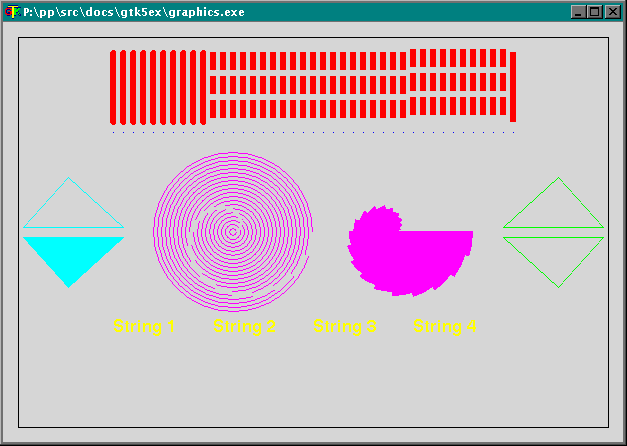
\epsfig{file=gtk5ex/graphics.png,width=\textwidth}
\end{figure}

\section{Animation}
The GDK drawing functions can be used to draw directly on a window visible
on the screen. This is OK for normal applications, but applications that
have a lot of (changing) graphics will soon see a flickering screen. 

Luckily, GDK provides a means to cope with this: Instead of drawing directly
on the screen, one can draw on a bitmap which exists in memory, and copy
parts of the bitmap to the screen on an as-need basis.

This is the reason why the GDK drawing functions generally accept a
\var{PGDKdrawable} parameter: This can be of the type \var{PgdkWindow} or
\var{PGDKPixmap}: The \var{TGDKPixmap} can be used to do the drawing in the
background, and then copy the pixmap to the actual window. 

This technique, known as double buffering, will be demonstrated in a small
arcade game: BreakOut. The game is quite simple: at the top of the screen,
there are a series of bricks. At the bottom of the screen is a small pad,
which can be move left or right using the cursor keys. A ball bounces on the
screen. When the ball hits a brick, the brick disappears. When the ball
hits the bottom of the window, the ball is lost. The pad can be used to
prevent the ball from hitting the bottom window.

When the pad hits the ball, the ball is accelerated in the direction the
pad was moving at the moment of impact. Also, an idea of 'slope' is
introduced: If the ball hits the pad at some distance from the pad's center,
the ball's trajectory is slightly disturbed, as if the pad has a slope.

After 5 balls were lost, the game is over. If all bricks have been
destroyed, a next level is started.

As stated above, the game will be implemented using double buffering.
The ball and pad themselves will be implemented as pixmaps; the bricks
will be drawn as simple rectangles.

These three objects will be implemented using a series of classes:
\var{TGraphicalObject}, which introduces a position and size. This class
will have 2 descendants: \var{TBlock}, which will draw a block on the
screen and \var{TSprite}, which contains all functionality to draw a moving
pixmap on the screen. From \var{TSprite}, \var{TBall} and \var{TPad} will be
derived. These two objects introduce the behaviour specific to the ball and
pad in the game.

The blocks will be managed by a \var{TBlockList} class, which is a
descendent of the standard \var{TList} class. 

All these objects are managed by a \var{TBreakOut} class, which contains the
game logic. The class structure could be improved a bit, but the idea is
more to separate the logic of the different objects.

The \var{TGraphicalObject} class is a simple object which introduces some 
easy access properties to get the position and size of the object:
\begin{lstlisting}{}
TGraphicalObject  = Class(TObject)
  FRect : TGdkRectangle;
Public 
  Function Contains(X,Y : Integer) : Boolean;
  Property Left : SmallInt Read FRect.x Write Frect.x;
  Property Top : SmallInt  Read FRect.y Write Frect.y;
  Property Width : Word  Read Frect.Width Write Frect.Width;
  Property Height : Word  Read Frect.Height Write Frect.Height;
end;
\end{lstlisting}{}

The \var{TBlock} object is a simple descendent of the \var{TGraphicalObject}
class:
\begin{lstlisting}{}
TBlock = Class(TGraphicalObject)
Private
  FMaxHits : Integer;
  FBlockList : TBlockList;
  FGC : PGDKGC;
  FColor : PGDKColor;
  FNeedRedraw : Boolean;
  Procedure CreateGC;
  Function DrawingArea : PGtkWidget;
  Function PixMap : PgdkPixMap; 
Public
  Procedure Draw;
  Function Hit : Boolean;
  Constructor Create (ABlockList : TBlockList);
  Property Color : PGDKColor Read FColor Write FColor;
end;
\end{lstlisting}{}
The \var{FMaxHits} field determines how many times the ball must hit the
brick before it disappears. With each hit, the field is decremented by 1.

The \var{FBlockList} refers to the blocklist object that will manage the 
block. The needed drawing widget and the pixmap on which the block must be
drawn are obtained from the blockmanager using the \var{DrawingArea} and 
\var{Pixmap} functions.
The \var{Draw} procedure will draw the block at it's position on the pixmap.
The \var{Color} property determines the color in which the block will be
drawn.

The implementation of the \var{TBlock} methods are quite simple. The first
methods don't need any explanation.
\begin{lstlisting}{}
Constructor TBlock.Create (ABlockList : TBlockList);

begin
  Inherited Create;
  FBlockList:=ABlockList;
  FMaxHits:=1;
end;

Function TBlock.DrawingArea : PGtkWidget;

begin
  Result:=FBlockList.FBreakout.FDrawingArea;
end;

Function TBlock.PixMap : PgdkPixMap; 

begin
  Result:=FBlockList.PixMap;
end;
\end{lstlisting}{}
The first interesting method is the \var{CreateGC} method:
\begin{lstlisting}{}
Procedure TBlock.CreateGC;

begin
  FGC:=gdk_gc_new(DrawingArea^.Window);
  gdk_gc_set_foreground(FGC,FColor);
  gdk_gc_set_fill(FGC,GDK_SOLID);
  FNeedRedraw:=True;
end;
\end{lstlisting}{}
The method is called the first time the block must be drawn. It allocates a
new graphics context using the \var{gdk\_gc\_new} function. This function
accepts a pointer to a \var{TGTKWidget} as a parameter and returns a new
graphics context. After the graphics context is created, the foreground
color and fill style are set. (it is assumed that \var{FColor} points
to a valid color)

The \var{Draw} procedure actually draws the block on the pixmap, using 
the graphics context created in the previous method:
\begin{lstlisting}{}
Procedure TBlock.Draw;

begin
  if FGC=Nil then
    CreateGC;
  if FNeedRedraw Then
    begin
    gdk_draw_rectangle(PGDKDrawable(Pixmap),FGC,-1,Left,Top,Width,Height);
    FNeedRedraw:=False;
   end;
end;
\end{lstlisting}{}
The \var{FNeedRedraw} procedure is used for optimization.

Finally, the \var{Hit} method is called when the block is hit by the ball.
It will decrease the \var{FMaxHits} field, and if it reaches zero, the 
place occupied by the block is redrawn in the background color. After that,
it removes itself from the blocklist and frees itself.
\begin{lstlisting}{}
Function TBlock.Hit : Boolean;

begin
  Dec(FMaxHits);
  Result:=FMaxHits=0;
  If Result then
    begin
    FBlockList.FBreakOut.DrawBackground(FRect);
    FBlockList.Remove(Self);
    Free;
    end;
end;
\end{lstlisting}{}

The \var{TSprite} object is a little more involved. The declaration is 
as follows:
\begin{lstlisting}{}
TSprite = Class(TGraphicalObject)
  FPreviousTop,
  FPreviousLeft : Integer;
  FDrawingArea : PGtkWidget;
  FDrawPixMap : PgdkPixmap;
  FPixMap : PgdkPixMap;
  FBitMap : PGdkBitMap;
Protected
  Procedure CreateSpriteFromData(SpriteData : PPGchar);
  Procedure CreatePixMap; Virtual; Abstract; 
  Procedure SavePosition;
Public
  Constructor Create(DrawingArea: PGtkWidget);
  Procedure Draw;    
  Function GetChangeRect (Var Rect : TGDkRectAngle) : Boolean;
  Property PixMap : PgdkPixMap Read FPixMap;
  Property BitMap : PGdkBitMap Read FBitMap; 
end;
\end{lstlisting}{}
The important property is the \var{PixMap} property; this contains the
pixmap with the sprite's image. The \var{BitMap} property contains the
bitmap associated with the pixmap. The second important method is the
\var{GetChangeRect} method; it returns the rectangle occupied by the
sprite at its previous position. This will be used to 'move' the sprite:
When moving the sprite, the current position is saved (using
\var{SavePosition}), and the new position is set. After that, the old 
position is cleared, and the sprite is drawn at the new position. 

All this drawing is done on the background pixmap, to avoid flickering 
when drawing: The result of the two drawing steps is shown at once.

The implementation of the \var{Draw} method is quite straightforward:
\begin{lstlisting}{}
Procedure TSprite.Draw;    

Var
  gc : PGDKGc;
  
begin
  if FPixMap=Nil then
    CreatePixMap;    
  gc:=gtk_widget_get_style(FDrawingArea)^.fg_gc[GTK_STATE_NORMAL];
  gdk_gc_set_clip_origin(gc,Left,Top);
  gdk_gc_set_clip_mask(gc,FBitmap);
  gdk_draw_pixmap(FDrawPixMap,gc,FPixMap,0,0,Left,Top,Width,Height)
  gdk_gc_set_clip_mask(gc,Nil);  
end;
\end{lstlisting}{}
After the pixmap has been created (a method which must be implemented by
descendent objects), the graphics context of the drawing area is retrieved 
to do the drawing.

The bitmap is drawn using the clipping functionality of the GDK toolkit:
To this end, the clip origin is set to the position of the sprite, and
the clip bitmask is set from the \var{FBitmap}, which is created when the
sprite's pixmap is created. When drawing the pixmap, only the bits in the
bitmap will be drawn, other bits are left untouched.

The pixmap is drawn using the \var{gdk\_draw\_pixmap} function. This
function copies a region from one \var{TGDKDrawable} to another.
It is defined as follows:
\begin{lstlisting}{}
procedure gdk_draw_pixmap(drawable:PGdkDrawable; gc:PGdkGC; 
                          src:PGdkDrawable; 
                          xsrc,ysrc,xdest,ydest,width,height:gint);
\end{lstlisting}{}
The function, as all GDK drawing functions, takes a \var{PGDKDrawable} 
pointer and a graphics contexts as its first two arguments. The third
argument is the \var{TGDKDrawable} which should be copied. The
\var{xsrc,ysrc} parameters indicate the position of the region that should
be copied in the source \var{TGDKDrawable}; the \var{xdest,ydest} indicate 
the position in the target \var{TGDKDrawable} where the bitmap should be
drawn.

In the case of \var{TSprite}, the function is used to copy the sprite's 
bitmap onto the memory pixmap with the game image. After the bitmap was
copied, the clip mask is removed again.

The creation of the pixmap happens when the sprite is drawn for the first
time; The \var{CreateSpriteFromData} method accepts a pointer to an XPM
pixmap, and uses the \var{gdk\_pixmap\_create\_from\_xpm\_d} function
(explained in the previous article) to create the actual pixmap and the 
corresponding bitmap.
\begin{lstlisting}{}
Procedure TSprite.CreateSpriteFromData(SpriteData : PPGChar);

begin
  FPixMap:=gdk_pixmap_create_from_xpm_d(FDrawingArea^.Window, 
                                        @FBitmap,
                                        Nil,
                                        SpriteData);
end;
\end{lstlisting}{}
This method can be used by the descendent object's \var{CreatePixmap} 
procedure.

The \var{SavePosition} and \var{GetChangeRect} methods are very
straightforward:
\begin{lstlisting}{}
Function TSprite.GetChangeRect (Var Rect : TGDkRectAngle) : Boolean;

begin
  Result:=(FPreviousLeft<>Left) or (FPreviousTop<>Top);
  If Result then
    With Rect do
      begin
      x:=FPreviousLeft;
      y:=FPreviousTop;
      Width:=Abs(Left-FPreviousLeft)+self.Width;
      height:=Abs(Top-FPreviousTop)+self.Height;
      end;
end;

Procedure TSprite.SavePosition;

begin
  FPreviousLeft:=Left;
  FPreviousTop:=Top;
end;
\end{lstlisting}{}
Note that the \var{GetChangeRect} procedure returns false if the position
of the sprite didn't change. This is used for optimization purposes.

The pad is the simplest of the two \var{TSprite} descendants. It only adds a
horizontal movement to the sprite:
\begin{lstlisting}{}
TPad = Class (TSprite)
Private
  FSlope,
  FSpeed,FCurrentSpeed : Integer;
Protected
  Procedure CreatePixMap; override;
  Procedure InitialPosition; 
Public  
  Constructor Create(DrawingArea: PGtkWidget);
  Procedure Step;
  Procedure GoLeft;
  Procedure GoRight;
  Procedure Stop;
  Property CurrentSpeed : Integer Read FCurrentSpeed;
  Property Speed : Integer Read FSpeed Write FSpeed;
  Property Slope : Integer Read FSlope Write FSlope;
end;
\end{lstlisting}{}
The procedures \var{GoLeft}, \var{GoRight} and \var{Stop} can be used to
control the movement of the pad. The method \var{Step} will be called at
regular intervals to actually move the pad. The \var{InitialPosition} 
sets the pad at its initial position on the screen. The \var{Speed} and 
\var{Slope} properties can be used to set the speed and slope of the pad.
The \var{Speed} is a number of pixels the pad will move per time unit.
The 'Slope' is a positive number. 

The implementation is quite straightforward:
\begin{lstlisting}{}
Constructor TPad.Create(DrawingArea: PGtkWidget);

begin
  Inherited Create(DrawingArea);
  FSpeed:=6;
  FSlope:=50;
end;

Procedure TPad.InitialPosition;

begin
  Left:=(FDrawingArea^.Allocation.Width-Width) div 2;
  Top:=FDrawingArea^.Allocation.Height-(2*Height);
  FCurrentSpeed:=0;
end;
\end{lstlisting}{}
The \var{InitialPosition} is used to reset the pad to its initial position
when the game starts, after a ball is lost or when a new level starts.

The various moving procedures do nothing except manipulate the current speed.
The handling here is quite simple, more complex handling (acceleration and
so on) could be handled.
\begin{lstlisting}{}
Procedure TPad.GoLeft;

begin
  FCurrentSpeed:=-FSpeed;
end;

Procedure TPad.GoRight;

begin
  FCurrentSpeed:=FSpeed;
end;

Procedure TPad.Stop;

begin
  FCurrentSpeed:=0;
end;
\end{lstlisting}{}
The pixmap for the pad is defined in a global constant \var{PadBitmap}. It is 
an array of \var{PCHar} which make up a XPM pixmap. The height and width of 
the bitmap are defined in global constants \var{PadHeight} and \var{PadWidth}
\begin{lstlisting}{}
Procedure TPad.CreatePixMap; 

begin
  CreateSpriteFromData(@PadBitmap[1]);
  Width:=PadWidth;
  Height:=PadHeight;
  InitialPosition;
end;
\end{lstlisting}{}
The \var{Step} method does the actual moving of the pad. It is called at regular intervals
by a timer. It saves the current position, and calculates the new position. A check is 
done for the boundaries of the game.
\begin{lstlisting}{}
Procedure TPad.Step;

begin
  SavePosition;
  Left:=Left+FCurrentSpeed;
  if Left<=0 then
    begin
    FCurrentSpeed:=-FCurrentSpeed;
    Left:=0;
    end
  else if Left+Width>=FDrawingArea^.allocation.width then
    begin
    FCurrentSpeed:=-FCurrentSpeed;
    Left:=FDrawingArea^.allocation.width-Width;
    end;
end;
\end{lstlisting}{}

The implementation of the \var{Tball} class is similar to the one of the \var{TPad},
only it introduces also a vertical speed. The speed of the ball is determined by 3 
numbers:
\begin{enumerate}
\item A horizontal speed.
\item A vertical speed. 
\item A speed factor. (a number between 0 and 100)
\end{enumerate} 
The sum of the absolute values of the vertical and horizontal speeds is always 100. 
To change the speed direction, the horizontal speed can be set to a value between 0
and 90. This means that the ball can never fly horizontally. The actual speed is 
determined by multiplying the horizontal speed and vertical speed with a speed 
factor. The 2 values that are obtained like that are the actual horizontal and 
vertical speed of the ball.

All this is implemented in the following class:
\begin{lstlisting}{}
TBall = Class (TSprite)
Private
  FBreakOut : TBreakOut;
  FCurrentSpeedX,
  FCurrentSpeedY : Integer;
  FSpeedfactor : Integer;
Protected
  Procedure CreatePixMap; override;
  Procedure SetSpeed(Value : Integer);
Public  
  Constructor Create(BreakOut : TBreakOut);
  Procedure Step;
  Procedure IncSpeed (Value: Integer);
  Procedure FlipSpeed (FlipX,FlipY : Boolean);
  Property CurrentSpeedX : Integer Read FCurrentSpeedX Write SetSpeed;
  Property CurrentSpeedY : Integer Read FCurrentSpeedY;
  Property SpeedFactor : Integer Read FSpeedFactor Write FSpeedFactor;
end;
\end{lstlisting}{}
The \var{FlipSpeed} method is used to change the ball's direction when it hits a brick
or one of the borders of the game. The \var{IncSpeed} method increases the speed of the
ball.

As usual, the implementation of these methods is quite straightforward;
\begin{lstlisting}{}
Constructor TBall.Create(BreakOut : TBreakOut);

begin
  Inherited Create(BreakOut.FDrawingArea);
  FBreakOut:=breakout;
  FCurrentSpeedY:=-100;
  FCurrentSpeedX:=0;
  FSpeedFactor:=10;
end;
\end{lstlisting}
The CreatePixmap uses the global constant \var{BallPixmap} to 
create the pixmap. The with and height are stored in the \var{BallWidth}
and \var{BallHeight} constants.
\begin{lstlisting}{}
Procedure TBall.CreatePixMap; 

begin
  CreateSpriteFromData(@BallBitmap[1]);
  Width:=BallWidth;
  Height:=BallHeight;
end;
\end{lstlisting}
The SetSpeed value is the write handler for the \var{CurrentSpeedX} property.
It makes sure that the value stays within certain bounds, and that the sum
of the horizontal and vertical speeds remains 100.
\begin{lstlisting}{}
Procedure TBall.SetSpeed(Value : Integer);

begin
  If Value<-FMaxXspeed then 
    Value:=-FMaxXSpeed
  else if Value>FMaxXspeed then
    Value:=FMaxXspeed;
  FCurrentSpeedX:=Value;
  If FCurrentSpeedY>0 then
    FCurrentSpeedY:=100-Abs(FCurrentSpeedX)
  else
    FCurrentSpeedY:=-100+Abs(FCurrentSpeedX);
end;
\end{lstlisting}
The \var{IncSpeed} procedure increases or decreases the speed of the ball, 
making sure it doesn't get smaller as 10.
\begin{lstlisting}{}
Procedure TBall.IncSpeed (Value: Integer);

begin
  FSpeedFactor:=FSpeedFactor+Value;
  If FSpeedFactor<10 then
    FSpeedFactor:=10;
end;

Procedure TBall.FlipSpeed (FlipX,FlipY : Boolean);

begin
  If FlipX then 
    FCurrentSpeedX:=-FCurrentSpeedX;
  If FlipY then 
    FCurrentSpeedY:=-FCurrentSpeedY;
end;
\end{lstlisting}
The last method of \var{TBall} is the \var{Step} method,
which moves the ball on the screen. It adjusts the speed when the ball hits the
border of the game area, and calls the \var{TBreakOut.LostBall} method
when the ball hits the bottom of the game area.
\begin{lstlisting}{}
Procedure TBall.Step;

begin
  SavePosition;
  Left :=Left + Round((FCurrentSpeedX*FSpeedFactor/100));
  Top  :=Top  + Round((FCurrentSpeedY*FSpeedFactor/100));
  if Left<=1 then
    begin
    FlipSpeed(True,False);
    Left:=1;
    end
  else if Left+Width>=FDrawingArea^.allocation.width then
    begin
    FlipSpeed(True,False);
    Left:=FDrawingArea^.allocation.width-Width-1;
    end;
  if Top<=1 then
    begin
    FlipSpeed(False,True);
    Top:=1;
    end
  else if Top+Height>=FDrawingArea^.allocation.Height then
    FBreakOut.LostBall
end;
\end{lstlisting}

\section{Game logic}
The previous objects were concerned with the graphical representation of the
game. The logic of the game is concentrated in 2 other objects: \var{TBlockList},
 which manages the blocks in the game, and \var{TBreakOut}, which implements the
game logic.

The \var{TBlockList} class is a simple descendent of \var{TList}:
\begin{lstlisting}{}
TBlockList = Class (TList)
  FTotalRows,FTotalColums,FStartRow,FBlockRows,FSpacing : Byte;
  FBreakOut : TBreakOut;
  FColor : PGDKColor;
  Function DRawingArea : PGTKWidget;
  FPixMap : PGDKPixmap;
Public 
  Constructor Create(BreakOut : TBreakOut);
  Destructor Destroy; override;
  Procedure CheckCollision (Ball: TBall);
  Procedure DrawBlocks;
  Procedure DrawBlocks(Const Area : TGdkRectangle);
  Procedure CreateBlocks;
  Procedure FreeBlocks;
  Property TotalRows : Byte Read FTotalRows Write FTotalRows;
  Property TotalColumns : Byte Read FTotalColums Write FTotalColums;
  Property StartRow : Byte Read FStartRow Write FStartRow;
  Property BlockRows : Byte Read FBlockRows Write FBlockRows;
  Property BlockSpacing : Byte Read FSpacing Write FSpacing; 
  Property PixMap : PGDKPixMap Read FPixMap Write FPixMap;
end;
\end{lstlisting}
It introduces some properties which control the look of the game:
\var{TotalRows}, \var{TotalColumns} is the total number of columns 
and rows in which blocks can be placed. \var{StartRow} and \var{BlockRows}
determines how many blocks are actually placed. \var{BlockSpacing} determines
the amount of space between the blocks. The \var{CheckCollision} determines
whether a ball has hit one of the blocks. The \var{DrawBlocks} draws only the blocks
that intersect with the rectangle defined in the \var{Area} parameter.
The other methods are self explaining.

The implementation of the \var{TBlockList} class is -as usual- quite simple:
\begin{lstlisting}{}
Constructor TBlockList.Create(BreakOut : TBreakOut);

begin
  FBreakOut:=BreakOut;
end;

Function TBlockList.DrawingArea : PGtkWidget;

begin
  Result:=FBreakOut.FDrawingArea;
end;

Destructor TBlockList.Destroy; 

begin
  If FColor<>Nil then
    FreeMem(FColor);
  FreeBlocks;
end;

Procedure TBlockList.DrawBlocks;

Var
  I : Longint; 

begin
  If Count=0 then
    CreateBlocks;
  For I:=0 to Count-1 do
    TBlock(Items[i]).draw;
end;

Procedure TBlockList.DrawBlocks (Const Area : TGdkRectangle);

Var
  i : longint;
  inters : TgdkRectangle;

begin
  For I:=0 to Count-1 do
    With TBlock(Items[i]) do
      FNeedRedraw:=gdk_rectangle_intersect(@area,@Frect,@inters)<>0;
  DrawBlocks;    
end;
\end{lstlisting}
The \var{gdk\_rectangle\_interset} returns 0 if 2 rectangles do not intersect,
and returns a nonzero constant if they do. If they do, the last parameter
is filled with the position and size of the intersecting rectangle.

\begin{lstlisting}{}
Procedure TBlockList.FreeBlocks;

Var
  I : longint;

begin
  For I:=Count-1 downto 0 do
    begin
    TBlock(Items[i]).Free;
    Delete(i);
    end;
end;
\end{lstlisting}
The \var{CreateBlocks} method creates the blocks and draws them on the screen.
It is called when the blocklist is drawn and there are no blocks.

The algorithm to color and place the blocks is quite simple, but a more 
complex algorithm that implements patterns of blocks depending on the 
level, and different colors for blocks could be implemented.
\begin{lstlisting}{}
Procedure TBlockList.CreateBlocks;

Var
  TotalHeight,TotalWidth,
  Cellheight,CellWidth,
  I,J : Integer;
  Block : TBlock;
  Min : Byte;
  
begin
  FColor:=AllocateColor(0,0,$ffff,DrawingArea);
  Min:=FSpacing div 2;
  If Min<1 then 
    Min:=1;
  TotalWidth:=Drawingarea^.Allocation.Width;
  TotalHeight:=DrawingArea^.Allocation.Height;
  Cellheight:=TotalHeight Div TotalRows;
  CellWidth:=TotalWidth div TotalColumns;
  For I:=StartRow to StartRow+BlockRows-1 do
    For J:=0 to TotalColumns-1 do
    begin
    Block:=TBlock.Create(Self);
    With Block do
      begin
      Top:=TotalHeight-(CellHeight*I)+Min;
      Left:=(CellWidth*J)+min;
      Width:=CellWidth-2*min;
      Height:=CellHeight-2*min;
      Color:=Self.FColor;
      FNeedRedraw:=True;
      end;
    add(Block);
    end;
end;
\end{lstlisting}
The checkcollision function checks all blocks to see whether it collides with the ball.
If so, it flips the speed of the ball and calls the balls \var{Hit} function. This will
remove the ball from the list if it is destroyed.

Note that the flipping of the speed of the ball checks where the ball came from, i.e.
looks at the previous position of the ball.
\begin{lstlisting}{}
Procedure TBlockList.CheckCollision (Ball: TBall);

var
  brect,ints : tgdkrectangle;
  B : TBlock;
  i : integer;
  flipx,flipy : Boolean;
    
begin
  For I:=Count-1 downto 0 do
    begin
    B:=TBlock(Items[i]);
    BRect:=B.FRect;    
    if gdk_rectangle_intersect(@Ball.Frect,@BRect,@ints)<>0 then
      begin
      FlipY:=((Ball.FpreviousTop>=(B.Top+B.Height)) and 
              (Ball.CurrentSpeedY<0)) or
             ((Ball.FpreviousTop+Ball.Height<=B.Top) and 
              (Ball.CurrentSpeedY>0));
      FlipX:=Not FlipY;
      If FlipX then
        FlipX:=((Ball.FPreviousLeft>=(B.Left+B.Width)) and 
                (Ball.CurrentSpeedX<0)) or
               (((Ball.FPreviousLeft+Ball.Width)<=B.Left) and 
                (Ball.CurrentSpeedX>0));
      Ball.FlipSpeed(FlipX,Flipy);
      if B.Hit and not (Count=0) then 
        gtk_widget_draw(DrawingArea,@BRect);
      Break;
      end;
    end;
end;
\end{lstlisting}

Finally, the \var{TBreakOut} class encapsulates the rest of the game logic. Its declaration 
is as follows:
\begin{lstlisting}{}
TBreakOut = Class(TObject)
Private
  FLevel : Integer;
  FBalls : Integer;
  FBGGC : PGDKGC;
  FBackGroundColor : PGDKColor;
  FPad : TPad;
  FBall : TBall;
  FBlockList : TBlockList;
  FDrawingArea : PGTKWidget;
  FPixMap : PGDKPixMap;
  Procedure DrawBackGround (Area : TGdkrectAngle);
  Procedure DrawBoard(Exposed : PGdkEventExpose);
  Procedure CreateGC;
  Procedure CreatePixMap;
  Procedure CopyPixMap(Area : TGdkRectangle);
  Procedure CheckCollision;
  Procedure FreeBall;
  Procedure NextLevel;
  Procedure NextBall;
  Procedure GameOver;
  Procedure LostBall;
  Procedure Redrawgame;
Public   
  Constructor Create (DrawingArea : PGtkWidget);
  Procedure Draw(Exposed : PGDKEventExpose);
  Procedure Step;
  Property BlockList : TBlockList Read FBlockList;
  Property Pad : TPad Read FPad;
  Property Level : Integer Read Flevel;
  Property Balls : Integer Read FBalls Write FBalls;
end;
\end{lstlisting}
The purpose of most of the methods of \var{TBreakOut} is self-evident. The \var{Draw}
method will be called when the drawing area on which the game is drawn is exposed.
The \var{Step} method will be called by a timer routine, and this will move all pieces
in the game, creating the illusion of movement. These are the only 2 public routines
of the component.

The constructor simply initializes the Ball and blocklist components. It does not
create a ball, this will be created when the ball enters the game.
\begin{lstlisting}{}
Constructor TBreakOut.Create (DrawingArea : PGtkWidget);

begin
  FDrawingArea:=DrawingArea;
  FBlockList:=TBlockList.Create (Self);
  FPad:=TPad.Create(FDrawingArea);
  FBalls:=5;
end;
\end{lstlisting}

The following routines are mainly concerned with the drawing of the various parts of the game.
\begin{lstlisting}{}
Procedure TBreakOut.DrawBoard(Exposed : PGdkEventExpose);

begin
  If FBGGC=Nil then
    CreateGC;  
  DrawBackGround(Exposed^.Area);
end;

Procedure TBreakOut.CreateGC;

begin
  FBGGC:=gdk_gc_new(FDrawingArea^.Window);
  FBackGroundColor:=AllocateColor(0,0,0,FDrawingArea);
  gdk_gc_set_foreground(FBGGC,FBackGroundColor);
  gdk_gc_set_fill(FBGGC,GDK_SOLID);
end;
\end{lstlisting}
The graphics context is needed for the drawing of the background of the game; 
it sets the drawing color to black and the fill style to solid. The graphics
context is then used in the \var{DrawBackground} method to draw the background
on the pixmap with the game image:
\begin{lstlisting}{}
Procedure TBreakOut.DrawBackGround (Area : TGdkrectAngle);

begin
  With Area do
    gdk_draw_rectangle(PGDKDrawable(FPixMap),FBGGC,-1,x,y,Width+1,Height+1);
end;
\end{lstlisting}
The pixmap that contains the game image is created the first time the breakout 
game is drawn. It is created using the \var{gdk\_pixmap\_new} function, which 
needs a \var{PGDKwindow} as the first parameter; from this window certain 
device properties are copied.

After the pixmap is created, it is assigned to the pad and blocklist objects.
\begin{lstlisting}{}
Procedure TBreakOut.CreatePixMap;

begin
  If FPixMap<>Nil then
    GDK_pixmap_unref(FPixMap);
  With FDrawingArea^ do
    FPixMap:=gdk_pixmap_new(Window,Allocation.Width,Allocation.Height,-1);
  FBlockList.PixMap:=FPixMap;
  FPad.FDrawPixMap:=FPixMap;
  If Assigned(FBall) then
    FBall.FDrawPixMap:=FPixMap;
end;
\end{lstlisting}
The following routine does the actual drawing of the screen: 
It copies the pixmap with the game image to the actual window. 
Not the whole pixmap is drawn (this would be very inefficient), 
but just the part indicated by the \var\var{Area} parameter.
\begin{lstlisting}{}
Procedure TBreakOut.CopyPixMap(Area : TGdkRectangle);

begin
  gdk_draw_pixmap(FDrawingArea^.Window,
                  gtk_widget_get_style(FDrawingArea)^.fg_gc[GTK_WIDGET_STATE(FDrawingArea)],
                  FPixMap,
                  area.x,area.y,
                  area.x,area.y,
                  area.width,area.height); 
end;
\end{lstlisting}
The \var{CopyPixmap} method is called as much as needed 
by the \var{Draw} method. This method tries to determine
the minimum amount of drawing needed to restore the game image on the screen.

It will draw the board, the exposed blocks, the previous position of
the ball and pad on the pixmap. After that the changed portions of
the pixmap are copied to the screen.
\begin{lstlisting}{}
Procedure TBreakOut.Draw(Exposed : PGDKEventExpose);

Var
  Rect : TGdkRectangle;

begin
  if FPixMap=Nil then 
    CreatePixMap;
  if Exposed<>Nil then
    begin
    DrawBoard(Exposed);
    FBlockList.DrawBlocks(exposed^.area)
    end
  else
    begin
    If Assigned(FBall) then 
      if FBall.GetChangeRect(Rect) then
        begin
        DrawBackground(Rect);
        FBLockList.drawBlocks(Rect);
        end;  
    if FPad.GetChangeRect(Rect) then
      DrawBackground(Rect)
    end;
  FPad.Draw;
  if Assigned(FBall) Then
    FBall.draw;
  If Exposed<>Nil then
    CopyPixMap(Exposed^.Area);
  If assigned(FBall) then
    if FBall.GetChangeRect(Rect) then
      CopyPixMap(Rect);
  if FPad.GetChangeRect(Rect) then
    CopyPixMap(Rect);
  IF Assigned(FBall) then
    CopyPixMap(FBall.FRect);
  CopyPixMap(FPad.FRect);
end;
\end{lstlisting}
The \var{RedrawGame} forces a redraw of the whole game, by forcing an expose event on the 
drawing area:
\begin{lstlisting}{}
Procedure TBreakout.Redrawgame;

Var
  Rect : TgdkRectangle;

begin
  Rect.X:=FDrawingArea^.allocation.x;
  Rect.Y:=FDrawingArea^.allocation.y;
  Rect.Width:=FDrawingArea^.allocation.Width;
  Rect.Height:=FDrawingArea^.allocation.Height;
  gtk_Widget_draw(FDrawingArea,@rect)
end;
\end{lstlisting}
The \var{Step} procedure is the central part of the game logic: it moves
the various components on the screen, and checks for collisions between 
the ball and the pad or the blocks. If a 'game over' or 'end of level' 
condition is detected, the appropriate methods are called to handle 
these situations.
\begin{lstlisting}{}
Procedure TBreakOut.Step;

begin
  FPad.Step;
  If Assigned(FBall) then
    FBall.Step;
  CheckCollision;
  If FBlockList.Count=0 then
    NextLevel;
  if Not Assigned(FBall) and (FBalls=0) then
    GameOver;
end;
\end{lstlisting}
The \var{CheckCollision} method checks for collisions of the ball with the pad
or with a block. The blocklist handles the collisions with a block, the collision
between the ball and the pad is handled here, in much the same was as it was handled
by the blocklist for the blocks. The only difference is that the speed of the ball 
is altered, depending on the speed of the pad:
\begin{enumerate}
\item If the pad was moving at the moment of impact, then the speed factor of
the ball is increased or decreased, depending on whether the ball and pad
 were moving in the same direction, or in opposite directions.
\item The angle of the ball is altered using the \var{Slope} of the pad. The horizontal
component of the speed is increased (or decreased) with a factor that depends on
the place where the ball hits the pad. If the pad is hit in the middle, no change takes
place. If it is not hit in the middle, the alteration is proportional to the distance
between the middle of the pad and the point of impact.
\end{enumerate}
\begin{lstlisting}{}
Procedure TBreakOut.CheckCollision;

Var
  Inters :TGdkrectangle;

begin
  If Assigned(FBall) then
   begin
   if gdk_rectangle_intersect(@FBall.FRect,@FPad.Frect,@inters)<>0 then
     If (FBall.FPreviousTop<FPad.Top) and (FBall.FCurrentSpeedY>0) then
       begin
       FBall.FlipSpeed(False,True);
       If (FPad.CurrentSpeed<>0) then
         if (FBall.FCurrentSpeedX*FPad.CurrentSpeed)>0 then
           FBall.IncSpeed(HitAccelleration)
         else
           FBall.IncSpeed(-HitAccelleration);
       FBall.CurrentSpeedX:=FBall.CurrentSpeedX+
                           (Round(((FBall.Left+(FBall.Width div 2)) - 
                                  (FPad.left+Fpad.Width div 2)) 
                                   * (FPad.Slope / 100)));
       end; 
   FBlockList.CheckCollision(FBall);  
   end;
end;
\end{lstlisting}
The following methods control the logic of the game. They are kept as simple
as possible, but they can be altered to make the game more interesting or 
visually attractive.
\begin{lstlisting}{}
Procedure TBreakOut.FreeBall;

begin
  FBall.Free;
  FBall:=Nil;
end;

Procedure TbreakOut.NextBall;

begin
  If FBall=Nil then
    begin
    FBall:=TBall.Create(Self);
    FBall.Top:=FPad.Top-1;
    FBall.Left:=FPad.Left + (FPad.Width div 2);
    FBall.CurrentSpeedX:=FPad.CurrentSpeed*5;
    FBall.FPreviousTop:=FBall.Top;
    FBall.FPreviousLeft:=FBall.Left;
    FBall.FDrawPixMap:=Self.FPixMap;
    FBall.Draw;
    end;
end;

Procedure TBreakOut.NextLevel;

Var
  Area : TGdkRectangle;

begin
  If Assigned(FBall) then
    FreeBall;
  FPad.FSpeed:=FPad.Speed+LevelAccelleration;
  FPad.InitialPosition;
  RedrawGame;
end;

Procedure TBreakout.LostBall;

begin
  Dec(FBalls);
  If FBalls=0 then 
    GameOver;
  FreeBall;
  Fpad.InitialPosition;
  RedrawGame;
end;

Procedure TBreakout.GameOver;

begin
end;
\end{lstlisting}

All the code for these three objects is collected in the unit \file{blocks}.

The main program uses the \var{TBreakOut} object to draw the game on a screen:
A simple, non-sizable window is created, and a \var{TGTKDrawingArea} widget is
dropped on it. A signal handler for the expose event of the widget is installed 
(the \var{Exposed} function), as well as a timeout which will step the game 
every 50 milliseconds (the \var{Step} function). After that, event handlers 
are installed for the keyboard, to the user can move the pad 
(the \var{KeyPress} function). The 'delete' event is also handled, to destroy the
window (the \var{Close} function).

The only logic in these functions consists of communicating the events to the 
\var{TBreakout} object, and to set the movement of the Pad based on the key 
that was hit. The program listing is presented without further comment.
\begin{lstlisting}{}
program breakout;

{$mode objfpc}

uses glib,gdk,gtk,blocks;

Type 
  TBreakOutWindow = Class(TObject)
  Public
    window, 
    area : PGtkWidget;
    BreakOut : TBreakOut;
  end;

Var
  GameWindow : TBreakOutWindow;
  
Function Close( widget : PGtkWidget ;
                event : PGdkEvent;
                data : gpointer) : boolean; cdecl;
Begin
  gtk_main_quit();
  Close := false;
End;

function Exposed(Widget: PGtkWidget;
                 event : PGdkEventExpose; 
                 Data : gpointer) : Integer; cdecl;

begin
  TBreakOutWindow(Data).BreakOut.Draw(Event);
  result:=0;
end;

function KeyPress (Widget: PGtkWidget;
                   event : PGdkEventKey; 
                   Data : gpointer) : Integer; cdecl;

begin
  with TBreakOutWindow(Data).BreakOut do
    Case event^.keyval of
      gdk_left  : Pad.Goleft;
      gdk_right : Pad.GoRight;
      gdk_down  : Pad.Stop;
      Ord(' ')  : NextBall;
    end;    
  Result:=0; 
end;

function Step (data : Gpointer): integer;cdecl;

Var
 Rect : TGdkRectangle;

begin
  With TBreakOutWindow(Data) do
    begin
    With Breakout do
      begin
      Step;
      Draw(Nil);
      end; 
    end;
  Result:=integer(True);
end;

Begin
  gtk_init( @argc, @argv );
  GameWindow:=TBreakOutWindow.Create;
  With GameWindow do
    begin
    window := gtk_window_new( GTK_WINDOW_TOPLEVEL );
    gtk_window_set_policy(PgtkWindow(Window),0,0,1);
    gtk_signal_connect(PGTK_OBJECT (window),'delete_event',
                       GTK_SIGNAL_FUNC(@Close),Nil);
    gtk_container_set_border_width (GTK_CONTAINER (window), 10);
    area := gtk_drawing_area_new();
    gtk_container_add( GTK_CONTAINER(window), Area);
    BreakOut:=TBreakOut.Create(area);
    With BreakOut.BlockList do
      begin
      TotalRows:=20;
      TotalColumns:=10;
      StartRow:=15;
      BlockRows:=5;
      BlockSpacing:=2;
      end;
    gtk_signal_connect (GTK_OBJECT (area),'expose_event',
                        GTK_SIGNAL_FUNC(@Exposed),GameWindow);
    gtk_drawing_area_size (PGTKDRAWINGAREA(area),600,400);
    gtk_widget_set_events(window,GDK_KEY_RELEASE_MASK);
    gtk_signal_connect(PGTKObject(Window),'key_press_event',
                       GTK_SIGNAL_FUNC(@KeyPress),GameWindow);
    gtk_timeout_add(50,@Step,GameWindow);
    gtk_widget_show_all(window); 
    gtk_main();
    end;
End.
  
end.
\end{lstlisting}
The result of the program can be seen in figure \ref{fig:breakout}.
\begin{figure}[ht]
\caption{The breakout program in action.}\label{fig:breakout}
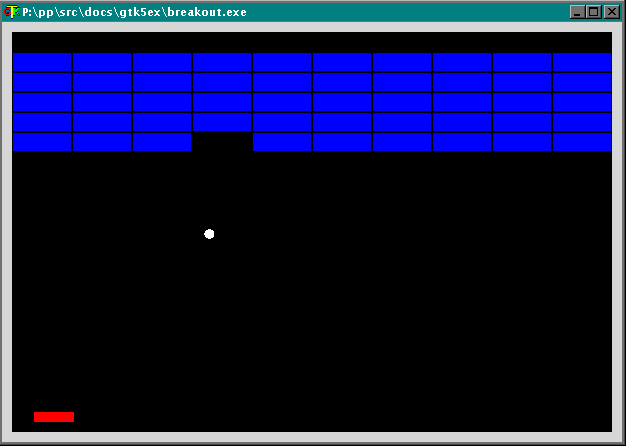
\epsfig{file=gtk5ex/breakout.png,width=\textwidth}
\end{figure}
The program can be enhanced in many ways:
\begin{enumerate}
\item More different colors for the blocks.
\item Different patterns of blocks when going to new levels.
\item Add some messages at the end of a level, or at game over.
\item Add a pause mode.
\item Add a menu to start/stop the game, and with some preferences
(game size, player level)
\item add a score based on the time it takes to finish a level.
\end{enumerate}
And many more things can probably be done. The program as it is now is playable, and 
fulfills it purpose: to demonstrate that simple game programming using the drawing 
facilities offered by GTK/GDK toolkit is possible and can be quite easy.
\end{document}
